\todo[inline, color=pink, size=normalsize]{Introdução da seção}

O pêndulo invertido é um sistema comumente empregado no ensino da teoria do Controle de Sistemas \cite{kelly_introduction_2017}. No entanto, a dinâmica associada ao pêndulo invertido pode ser empregada na modelagem da caminhada de robôs humanoides \cite{venancio_desenvolvimento_2018}, no estudo da dinâmica de foguetes durante o lançamento \cite{peltroche_advanced_2019}, e no controle de veículos do tipo \textit{Segway}\textsuperscript{\textregistered} \cite{younis_design_2009}.  

Para fins de aplicação considere o pêndulo invertido apresentado na Figura \ref{fig:penduloInvertido:variaveis}. Este é composto por um carro que, impulsionado por um motor, se move ao longo de um trilho e por um pêndulo que pende livremente desse carro. O ângulo entre o pêndulo e a vertical é dado por $ \theta(t) $, enquanto $ \omega(t) $ e $ l $ são a velocidade angular do pêndulo e o comprimento de sua haste. A distância entre o carro e o centro do trilho é dada por $ d(t) $, enquanto $ v(t) $ é a velocidade do carro, $ F(t) $ é a força que o impulsiona, $ m_1 $ e $ m_2 $ são as massas do carro e do pêndulo, respectivamente, e $ g $ é a aceleração da gravidade \cite{kelly_introduction_2017}.

\noindent	
\begin{minipage}{\textwidth}
	\vspace{\onelineskip}
	\centering
	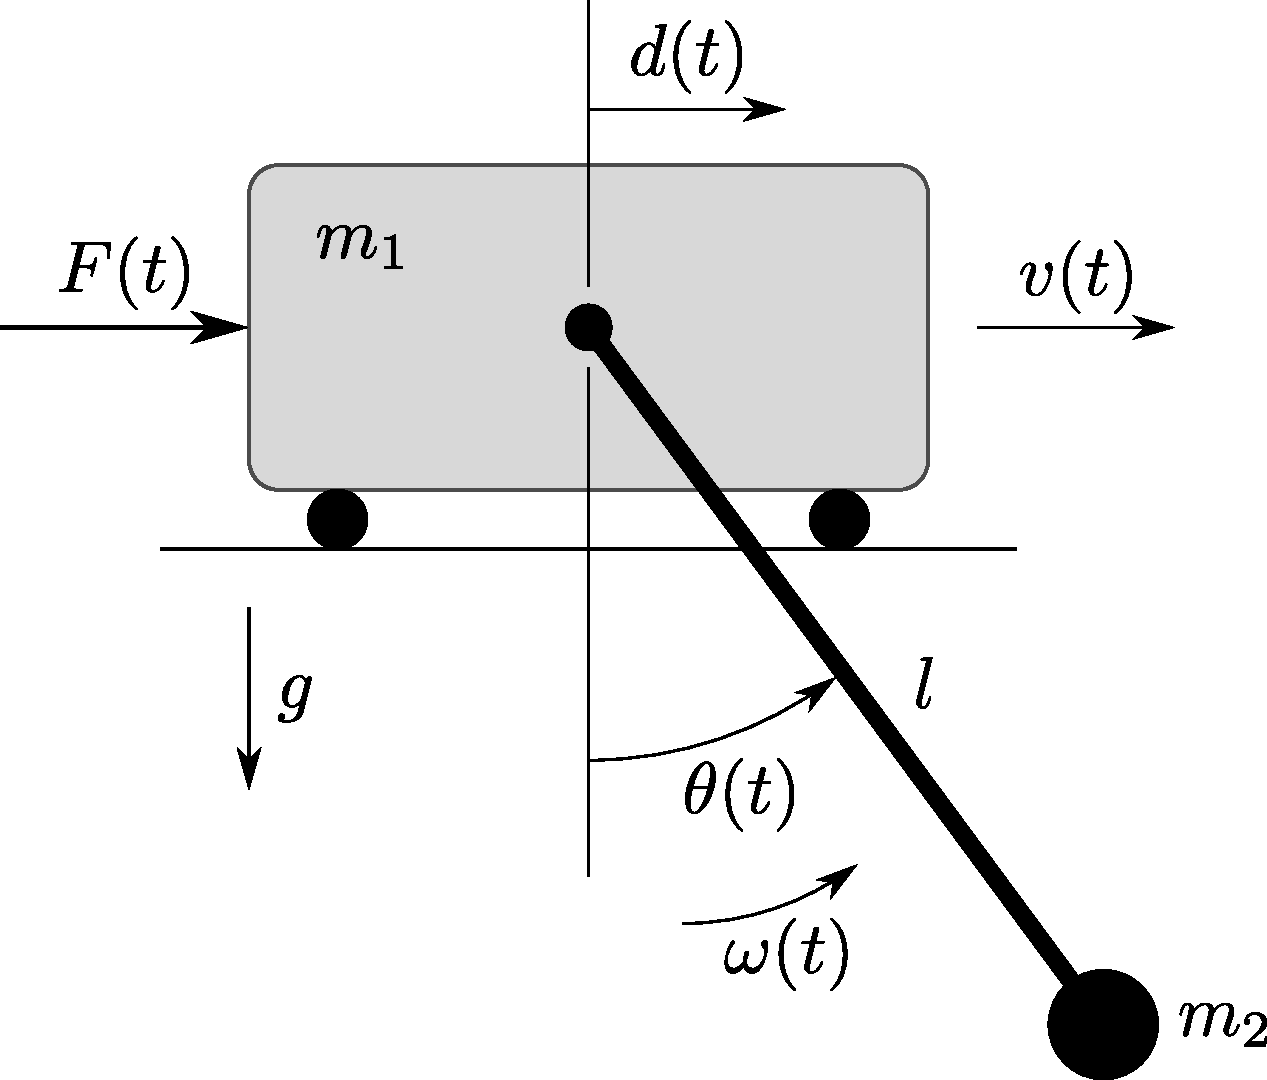
\includegraphics[scale=0.3]{draw/resultados/pdf/pendulo}
	\captionof{figure}[Representação esquemática de um pêndulo invertido]{Representação esquemática de um pêndulo invertido e das variáveis utilizadas na descrição da dinâmica desse sistema.}
	\label{fig:penduloInvertido:variaveis}
	\vspace{\onelineskip}
\end{minipage}

Neste estudo deseja-se determinar a trajetória a ser percorrida pelo um pêndulo invertido para que o mesmo realize uma manobra de balanço ascendente (\textit{swing-up}), empregando o mínimo esforço. Inicialmente em repouso, o carro deve partir do centro do trilho, com a haste do pêndulo pendendo na vertical, e se movimentar de forma que a posição $ d_f $ seja atingida $ t_f $ segundos após o início da manobra, ao mesmo tempo em que a haste do pêndulo, apontando agora para cima, atinge a posição vertical, conforme ilustrado na Figura \ref{fig:penduloInvertido:penduloInicialFinal} \cite{kelly_introduction_2017}. 

\noindent	
\begin{minipage}{\textwidth}
	\vspace{\onelineskip}
	\centering
	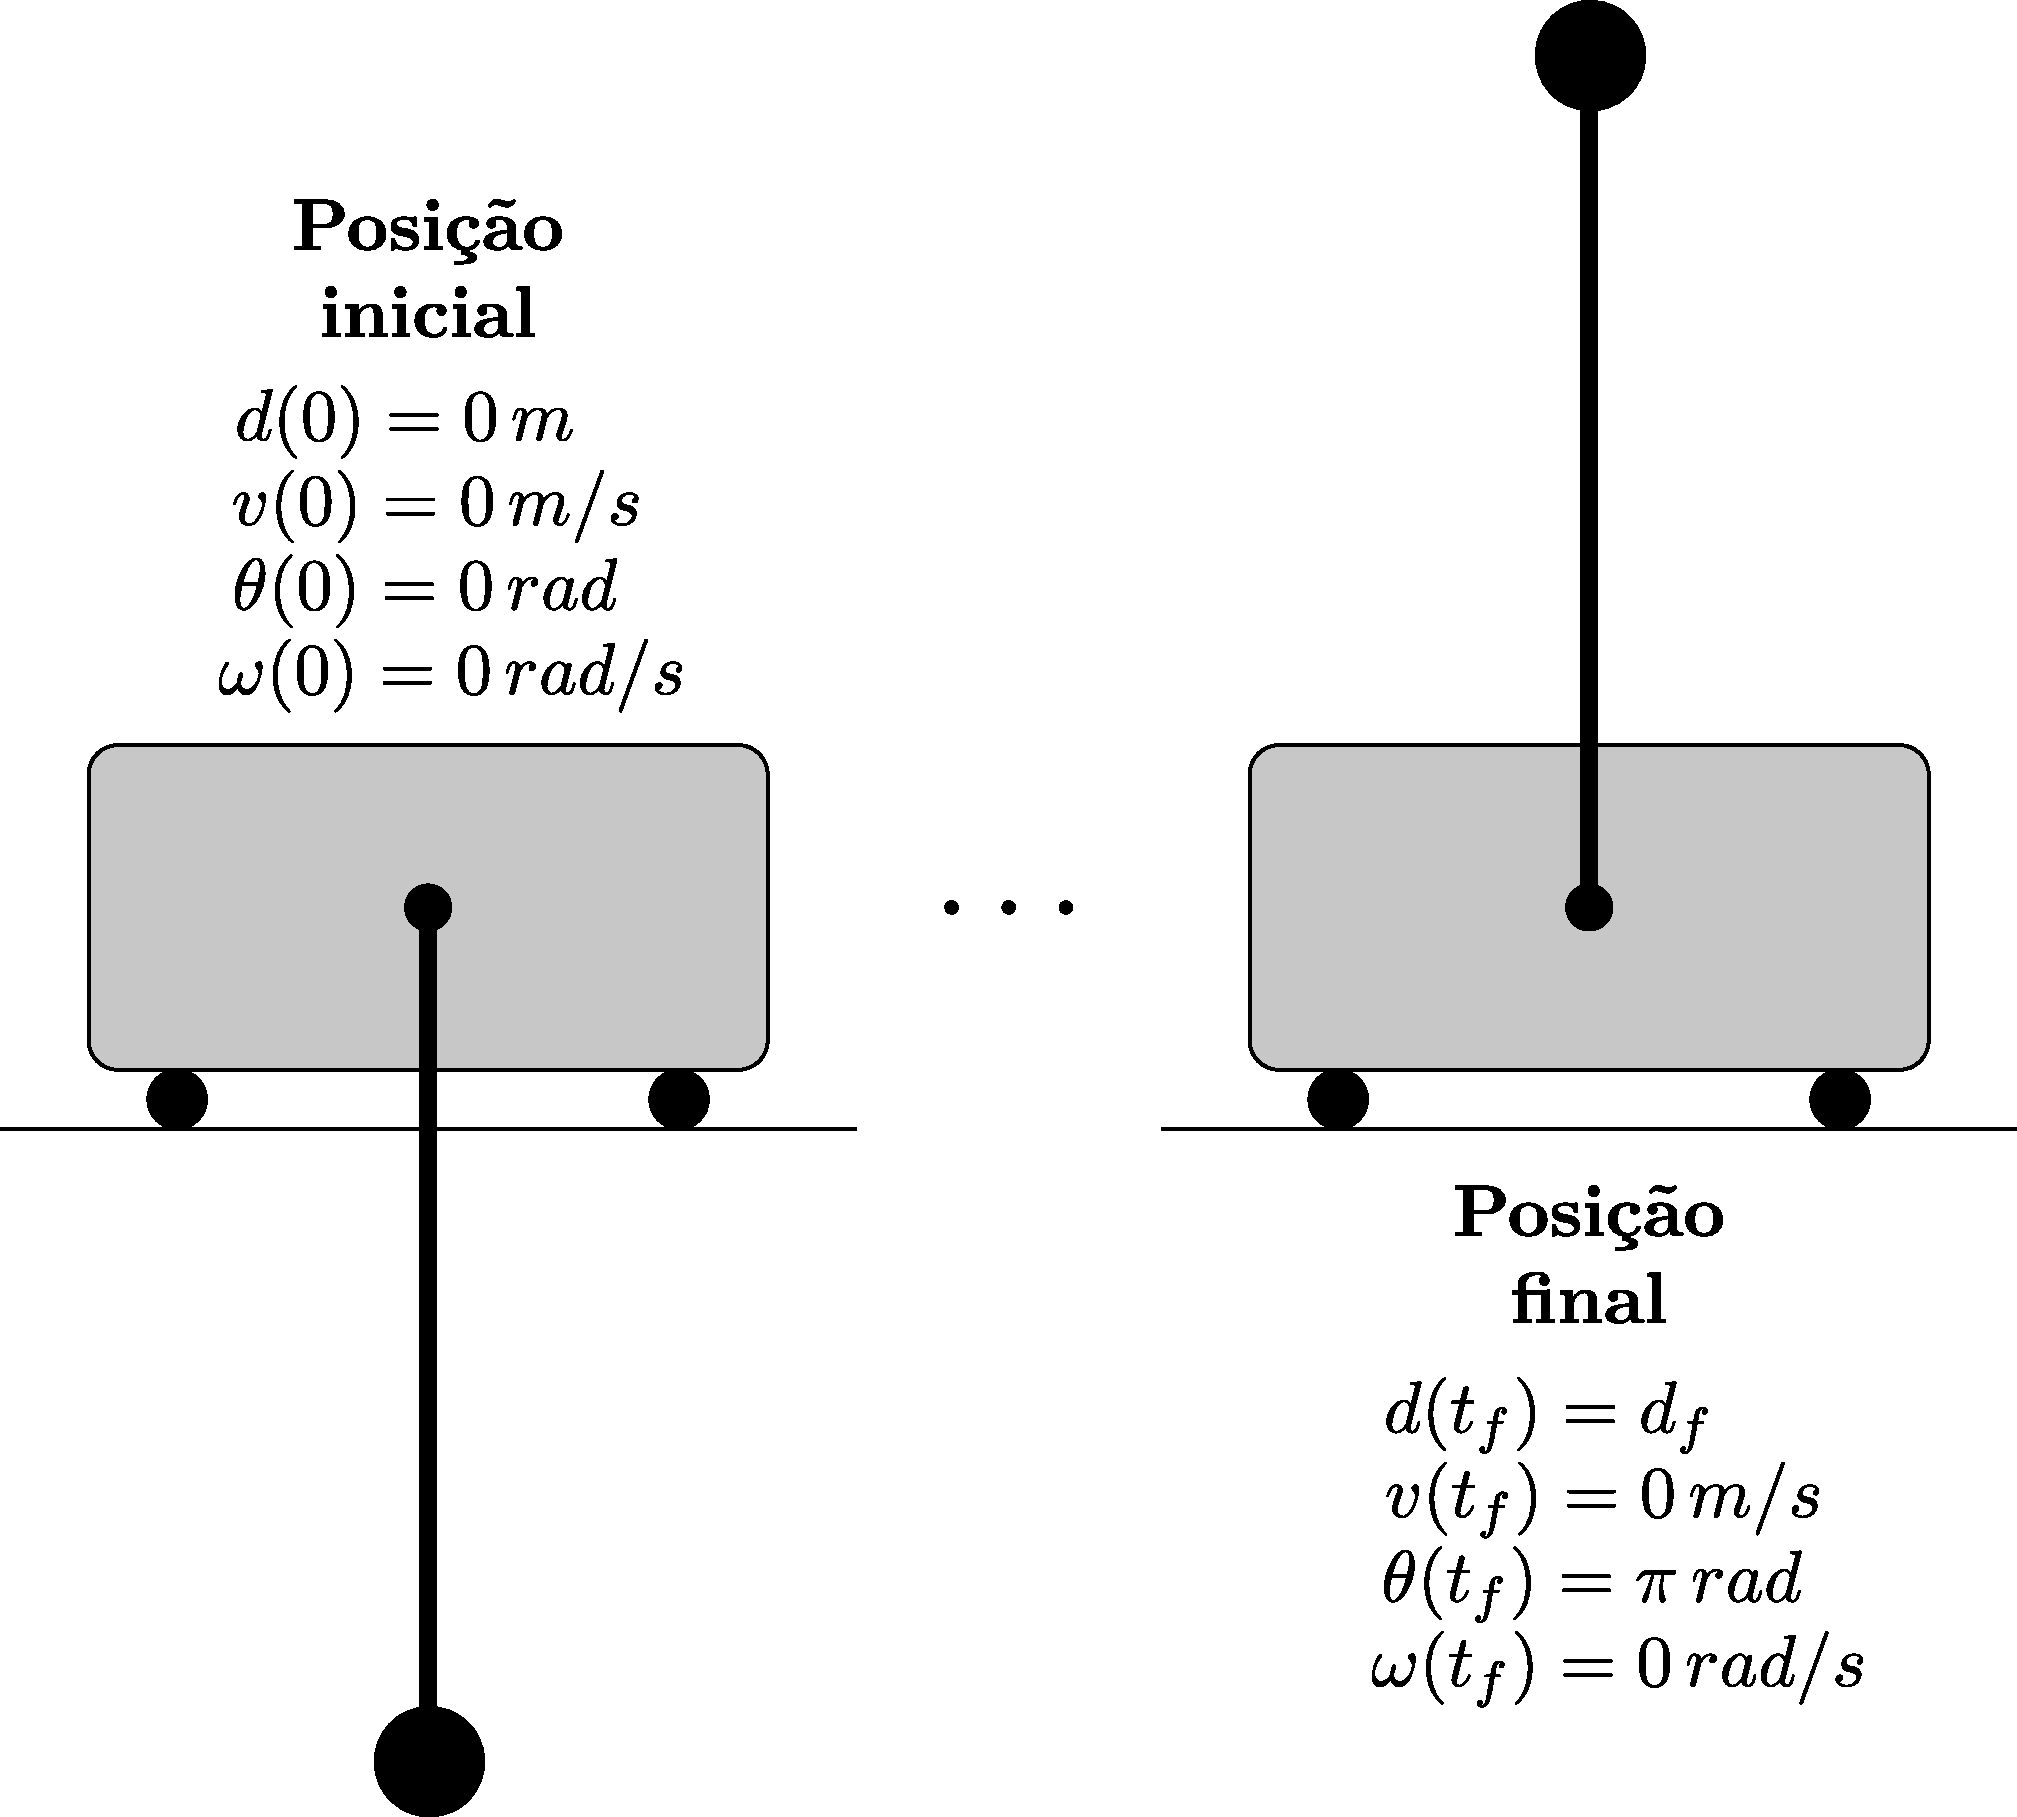
\includegraphics[scale=0.3]{draw/resultados/pdf/penduloInicialFinal}
	\captionof{figure}[Posições inicial e final definidas pra o problema do pêndulo invertido]{Posições inicial e final definidas para o problema do pêndulo invertido durante a execução da manobra de \textit{swing-up}.}
	\label{fig:penduloInvertido:penduloInicialFinal}
	\vspace{\onelineskip}
\end{minipage}

\todo[inline, color=pink, size=normalsize]{Função objetivo}

Para este estudo de caso deseja-se minimizar a função objetivo descrita como \cite{kelly_introduction_2017}:
%
\begin{equation}
	\label{eq:penduloInvertido:J}
	J = \int_{0}^{t_f} F^2(t) dt
\end{equation}
%
sujeito as seguintes restrições:
%
\begin{subequations}
\begin{equation}
\label{eq:penduloInvertido:dinamica}
\dot{d}(t) = v(t),\;\;d(0) = 0 \; \text{m}
\end{equation}
\vspace{-0.75cm}
\begin{equation}
\dot{\theta}(t) = \omega(t),\;\;\theta(0) = 0 \; \text{rad}
\end{equation}
\vspace{-0.75cm}
\begin{equation}
\dot{v}(t) = \frac{l \, m_2 \, \omega^2(t) \, sen \big(\theta(t)\big) + F(t) + m_2 \, g \, cos \big(\theta(t)\big) \, sen\big(\theta(t)\big)}{m_1 + m_2 \big[1 - cos^2 \big(\theta(t) \big)\big]},\;\;v(0) = 0 \; \text{m/s} 
\end{equation}
\vspace{-0.6cm}
\begin{equation}
\dot{\omega}(t) = -\frac{l \, m_2 \, \omega^2(t) \, sen\big(\theta(t)\big) \, cos\big(\theta(t)\big) + F(t) \, cos\big( \theta(t) \big) + (m_1 + m_2) g \, sen\big(\theta(t)\big)}{l \, m_1 + l \, m_2 \big[1 - cos^2\big(\theta(t)\big) \big]},\nonumber
\end{equation}
\vspace{-0.6cm}
\begin{equation}
\omega(0) = 0 \, \text{rad/s}
\end{equation}
\end{subequations}
%
em que $ \mathbf{x}(t) = \begin{bmatrix} d(t) & \theta(t) & v(t) & \omega(t) \end{bmatrix}^T $ é o vetor de variáveis de estados e $ F(t) $ é a variável de controle. 

Uma vez que o trilho sobre o qual o carro se movimenta é finito e levando em conta que há um limite associado à força que o motor pode impor sobre o carro, devem-se considerar as restrições:
%
\begin{subequations}
\begin{equation}
\label{eq:penduloInvertido:laterais}
-d_{max} \leq d(t) \leq d_{max}
\end{equation}
\vspace{-0.5cm}
\begin{equation}
-F_{max} \leq F(t) \leq F_{max}
\end{equation}
\end{subequations}
%
sendo $ d_{max} $ a metade da extensão do trilho e $ F_{max} $ a máxima força que pode ser imposta pelo motor. 

Também são impostas restrições terminais, definidas como segue:
%
\begin{subequations}
\begin{equation}
\label{eq:penduloInvertido:terminais}
d(t_f) = d_f\; \text{m}
\end{equation}
\vspace{-0.85cm}
\begin{equation}
\theta(t_f) = \theta_f\; \text{rad}
\end{equation}
\vspace{-0.7cm}
\begin{equation}
v(t_f) = 0\; \text{m/s}
\end{equation}
\vspace{-0.75cm}
\begin{equation}
\omega(t_f) = 0\;\text{rad/s}
\end{equation}
\end{subequations}

Os parâmetros empregados neste estudo de caso são \cite{kelly_introduction_2017}: aceleração da gravidade ($ g = 9,81 $ m/s$^2$), massa do carro ($ m_1 = 1$ kg), massa do pêndulo ($ m_2 = 0,3 $ kg), comprimento da haste do pêndulo ($ l = 0,5 $ m), tempo final ($ t_f = 2 $ s), distância percorrida pelo carro ao longo da execução da manobra ($ d_f = 1 $ m), posição angular final do pêndulo ($ \theta_f = \pi $ rad), máxima força que pode ser imposta pelo motor que impulsiona o carro ($ F_{max} = 20 $ N), e metade do comprimento do trilho sobre o qual o carro se movimenta ($ d_{max} = 2 $ m).

\todo[inline, color=pink, size=normalsize]{Observações sobre a inicialização dos estados e controles}

Para que as trajetórias das variáveis de estado e de controle obtidas pela metodologia proposta se assemelhem à aquelas reportadas em \citeonline{kelly_introduction_2017}, assume-se, \textit{a priori}, que os estados do sistema evoluem linearmente ao longo da execução da manobra de \textit{swing-up} e que $ F(t) $ permanece nulo para $ t \in [0, \, t_f] $. Assim sendo, para resolução do estudo de caso em análise por meio do $ COPILOTS $ adotou-se as seguintes estimativas iniciais \cite{kelly_introduction_2017}:
%
\begin{subequations}
\begin{equation}
\label{eq:penduloInvertido:palpites}
x_p(t) = \frac{t}{t_f} \begin{bmatrix} d_f & \pi & 0 & 0 \end{bmatrix}^T 
\end{equation}
\vspace{-0.75cm}
\begin{equation}
u_p(t) = 0
\end{equation}
\end{subequations}
%
sendo $ x_p(t) $ e $ u_p(t) $ as estimativas iniciais para os perfis de estado e controle, respectivamente. 

\todo[inline, color=pink, size=normalsize]{Introdução da análise de sensibilidade $ J \times N $}

São apresentados na Figura \ref{fig:penduloInvertido:sensibilidade:J} a influência do número de nós de colocação $N$ no valor da função objetivo (melhor solução obtida), bem como o número de pontos mínimo $N_m$ encontrados por cada abordagem. Para essa análise foram escolhidos 30 valores igualmente espaçados e pertencentes ao intervalo [5 92].

\noindent	
\begin{minipage}{\textwidth}
	\vspace{\onelineskip}
	\centering
	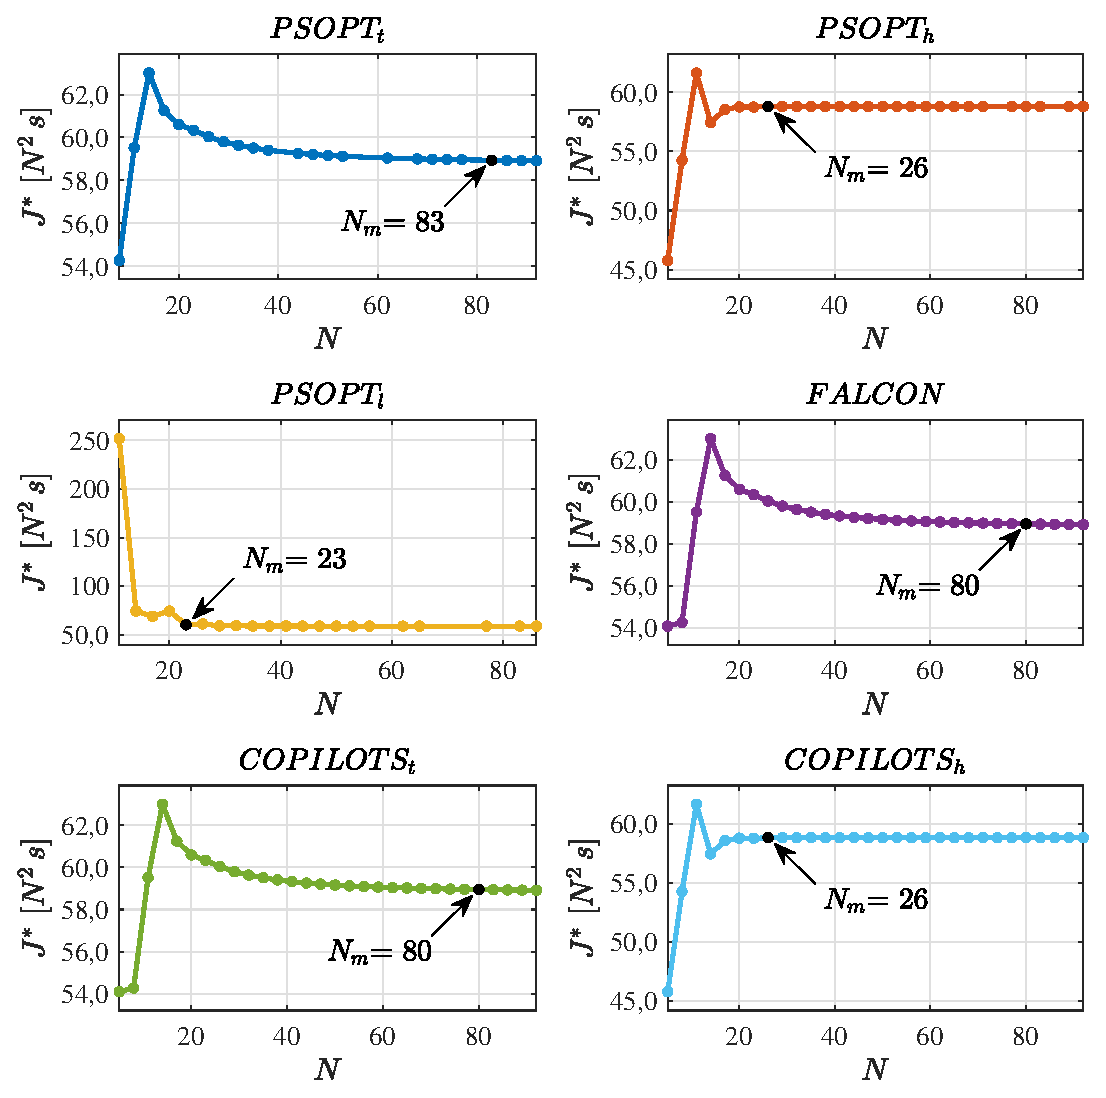
\includegraphics[scale=0.7]{fig/resultados/penduloInvertido/sens/J}
	\captionof{figure}[Influência do número de nós de colocação no valor da função objetivo para o problema do pêndulo invertido]{
	Influência do número de nós de colocação $ N $ no valor da função objetivo $ J^* $ para o problema do pêndulo invertido.}
	\label{fig:penduloInvertido:sensibilidade:J}
	\vspace{\onelineskip}
\end{minipage}

\todo[inline, color=pink, size=normalsize]{Análise dos gráficos $ J \times N $}

Nesta figura observa-se que, após um determinado valor para $N_m$, todos os pacotes convergiram para a solução reportada na literatura (\textcolor{red}{Inserir por favor o valor da função objetivo e a referência}). Todavia, deve ser mencionado que não foi possível, empregando o $ PSOPT_t $, o $ PSOPT_h $ e o $ PSOPT_l $, obter soluções para todos os $ N $ considerados. Em contrapartida, o valor de $ J^* $ para o $ PSOPT_l $ convergiu mais rapidamente que aqueles requeridos pelas outras abordagens. Os valores entre $ J^* $ e $ N $ associadas a cada um dos métodos que fazem uso de colocação trapezoidal ($ FALCON $, o $ PSOPT_t $ e $ COPILOTS_t $) foram semelhantes entre si. Esta concordância pode ser verificada quando comparam-se os resultados obtidos peplo $ PSOPT_h $ e $ COPILOTS_h $, ambos métodos que empregam a colocação Hermite-Simpson. Além disso, observa-se que os valores de  $ J^* $ referentes aos métodos que empregam a colocação trapezoidal aumentam até atingir seu valor máximo e depois voltam a cair até alcançar a convergência, estando o pico de $ J^* $ associado a $ N = 14 $. Nesse caso, escolheu-se $ N_m $ utilizando a métrica proposta originalmente, porém, desconsiderando-se os $ J^* $ obtidos para $ N < 14 $. De forma análoga, observa-se que os $ J^* $ associados aos métodos que fazem uso da colocação Hermite-Simpson crescem até $ N = 11 $, depois sofrem uma queda brusca em $ N = 14 $, para em seguida voltarem a crescer lentamente até atingir a convergência. Para estes casos considera-se que esse no aumento no valor da função objetivo se deve ao pequeno número de nós de colocação associado à violações nas restrições, o que implica em valores de $J$ não coerentes com o reportado \cite{kelly_introduction_2017}. Assim como observado para o problema anterior, ressalta-se a importância da realização de análise de sensibilidade no que tange o número de nós de colocação, bem como da análise do atendimento das restrições do estudo em questão.

\todo[inline, color=pink, size=normalsize]{Introdução dos resultados $ N = N_m $}

As métricas calculadas por cada um dos pacotes são apresentadas Tabela \ref{tab:penduloInvertido:raw} considerando $N=N_m$. Nesta tabela tem-se o valor da função objetivo ($ J^* $), o tempo de processamento médio ($ t_p $), o desvio padrão atribuído ($ s_t $), a máxima violação das restrições ($ \Delta c_{max} $) e o número de execuções bem sucedidas ($ N_s $).

\begin{table}[!h]
	\centering
	\caption[Métricas  obtidas  para  o  problema  do pêndulo invertido]{Métricas  obtidas  para  o  problema  do pêndulo invertido. Os melhores $ N_m $, $ J^* $, $ t_p $, $ n_{aval} $ e $ N_s\% $ se encontram destacados.}
	\label{tab:penduloInvertido:raw}
	\begin{tabular}{@{}ccccccccc@{}}
		\toprule
		Método       & $N_m$                              & $J^*$                                    & $t_p$ {[}$s${]}                         & $s_t$ {[}$s${]} & $n_{aval}$                         & $\Delta c_{max}$                         & $N_s$ & $N_s\%$                                  \\ \midrule
		$PSOPT_t$    & 83                                 & 58,93880                                 & 1,86743                                 & 0,18145         & 542                                & 4,32e-14                                 & 24    & 80,00\%                                  \\
		$PSOPT_h$    & 26                                 & {\color[HTML]{009901} \textbf{58,80540}} & 0,59690                                 & 0,04756         & 221                                & 2,78e-14                                 & 28    & 93,33\%                                  \\
		$PSOPT_l$    & {\color[HTML]{009901} \textbf{23}} & 60,16670                                 & 0,43817                                 & 0,01904         & 47                                 & 6,64e-14                                 & 21    & 70,00\%                                  \\
		$FALCON$     & 80                                 & 58,94871                                 & {\color[HTML]{009901} \textbf{0,18535}} & 0,03597         & {\color[HTML]{009901} \textbf{34}} & 9,32e-11                                 & 30    & {\color[HTML]{009901} \textbf{100,00\%}} \\
		$COPILOTS_t$ & 80                                 & 58,94871                                 & 16,46423                                & 0,08403         & 27044                              & 1,55e-15 & 30    & {\color[HTML]{009901} \textbf{100,00\%}} \\
		$COPILOTS_h$ & 26                                 & 58,80543                                 & 17,42163                                & 0,63533         & 34017                              & 2,28e-15                                 & 30    & {\color[HTML]{009901} \textbf{100,00\%}} \\ \bottomrule
	\end{tabular}
\end{table}

\todo[inline, color=pink, size=normalsize]{Análise dos resultados $ N = N_m $}

Nesta tabela é possível observar que os valores de $ N_m $ relacionados aos métodos que fazem uso da colocação trapezoidal ($ FALCON $, $ PSOPT_t $ e $ COPILOTS_t $)  se mostraram bem próximos uns dos outros e bem maiores que os computados pelos demais métodos. O $ PSOPT_l $ foi o que resultou no menor valor para $ N_m $. Já o maior valor de função objetivo foi encontrado pelo $ PSOPT_l $. Apesar do elevado valor de $ N_m $ requerido pelo $ FALCON $, verifica-se que a esse não está diretamente associado os menores valores de $ t_p $ e de $ n_{aval} $. Os valores de $ t_p $ e de $ n_{aval} $ associados ao $ COPILOTS $, independentemente do tipo de colocação considerado, são bem maiores que os requeridos pelos demais pacotes. Em contrapartida, verifica-se que o $ COPILOTS_h $ e o $ PSOPT_h $ convergiram para valores próximos ao melhor encontrado. O parâmetro $ N_m $ requerido pelo $ COPILTS_h $ é cerca de três vezes menor que o associado ao $ COPILOTS_t $. Ainda assim, o $ COPILOTS_h $ requeriu um valor de $ n_{aval} $ menor com relação ao $ COPILOTS_t $. Finalmente, ressalta-se que somente o $ FALCON $ e o $ COPILOTS $ foram capazes de encontrar a solução para todos os valores de $ N $ considerados. 

\todo[inline, color=pink, size=normalsize]{Introdução das trajetórias}

Os perfis referentes as variáveis de estado e controle considerando $ N = N_m $ são apresentadas nas Figuras \ref{fig:penduloInvertido:x:d}-\ref{fig:penduloInvertido:u:F}. 
Nestas figuras é possível observar boa concordância entre todos os perfis. A única trajetória de controle um pouco discrepante foi obtida pelo $ PSOPT_l $, em que são observadas pequenas oscilações no início e no fim da trajetória. Esse comportamento pode estar relacionado como é realizada a interpolação da trajetória de controle neste pacote.

\noindent
\begin{minipage}{\textwidth}
	\vspace{\onelineskip}
	\centering
	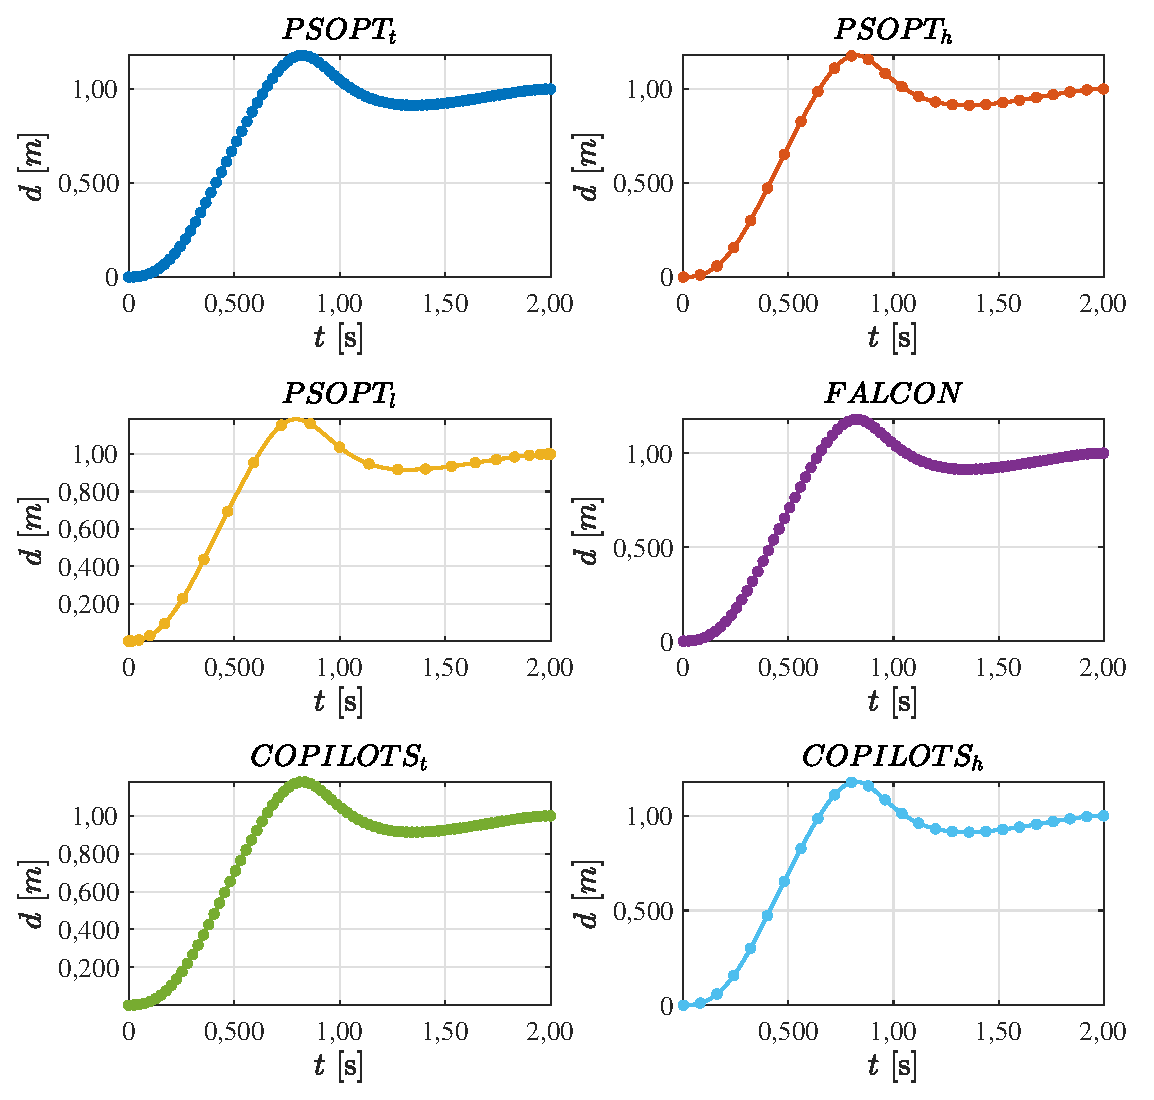
\includegraphics[scale=0.7]{fig/resultados/penduloInvertido/traj/x/d}
	\captionof{figure}[Variável de estado $d(t)$ para o problema do pêndulo]{Variável de estado $d(t)$ para o problema do pêndulo. Os pontos representam os valores discretizados e as linhas contínuas representam as trajetórias interpoladas.}
	\label{fig:penduloInvertido:x:d}
	\vspace{\onelineskip}
\end{minipage}

\noindent
\begin{minipage}{\textwidth}
	\vspace{\onelineskip}
	\centering
	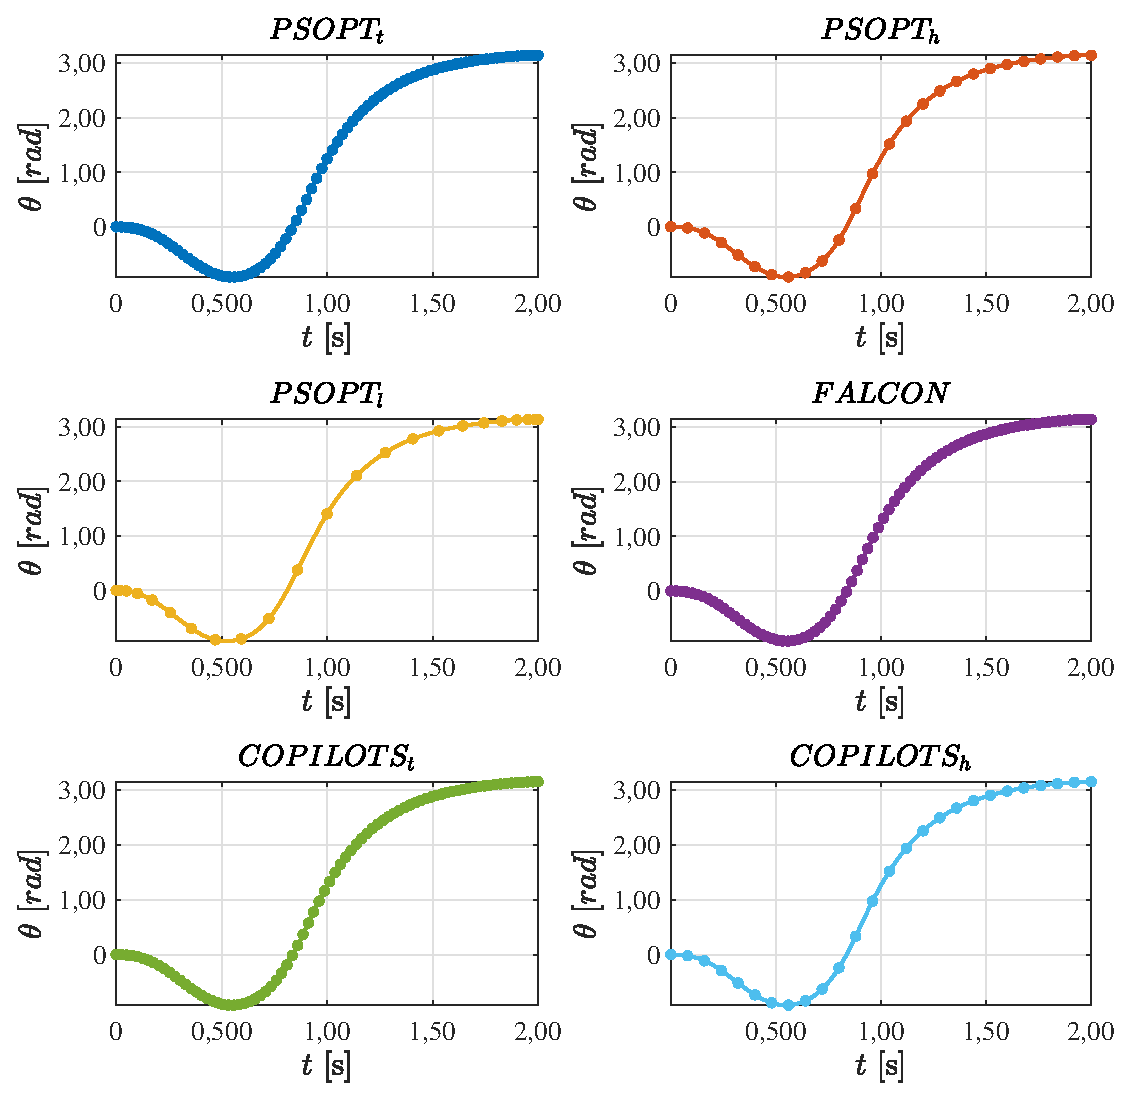
\includegraphics[scale=0.7]{fig/resultados/penduloInvertido/traj/x/theta}
	\captionof{figure}[Variável de estado $\theta(t)$ para o problema do pêndulo]{Variável de estado $\theta(t)$ para o problema do pêndulo. Os pontos representam os valores discretizados e as linhas contínuas representam as trajetórias interpoladas.}
	\label{fig:penduloInvertido:x:theta}
	\vspace{\onelineskip}
\end{minipage}

\noindent
\begin{minipage}{\textwidth}
	\vspace{\onelineskip}
	\centering
	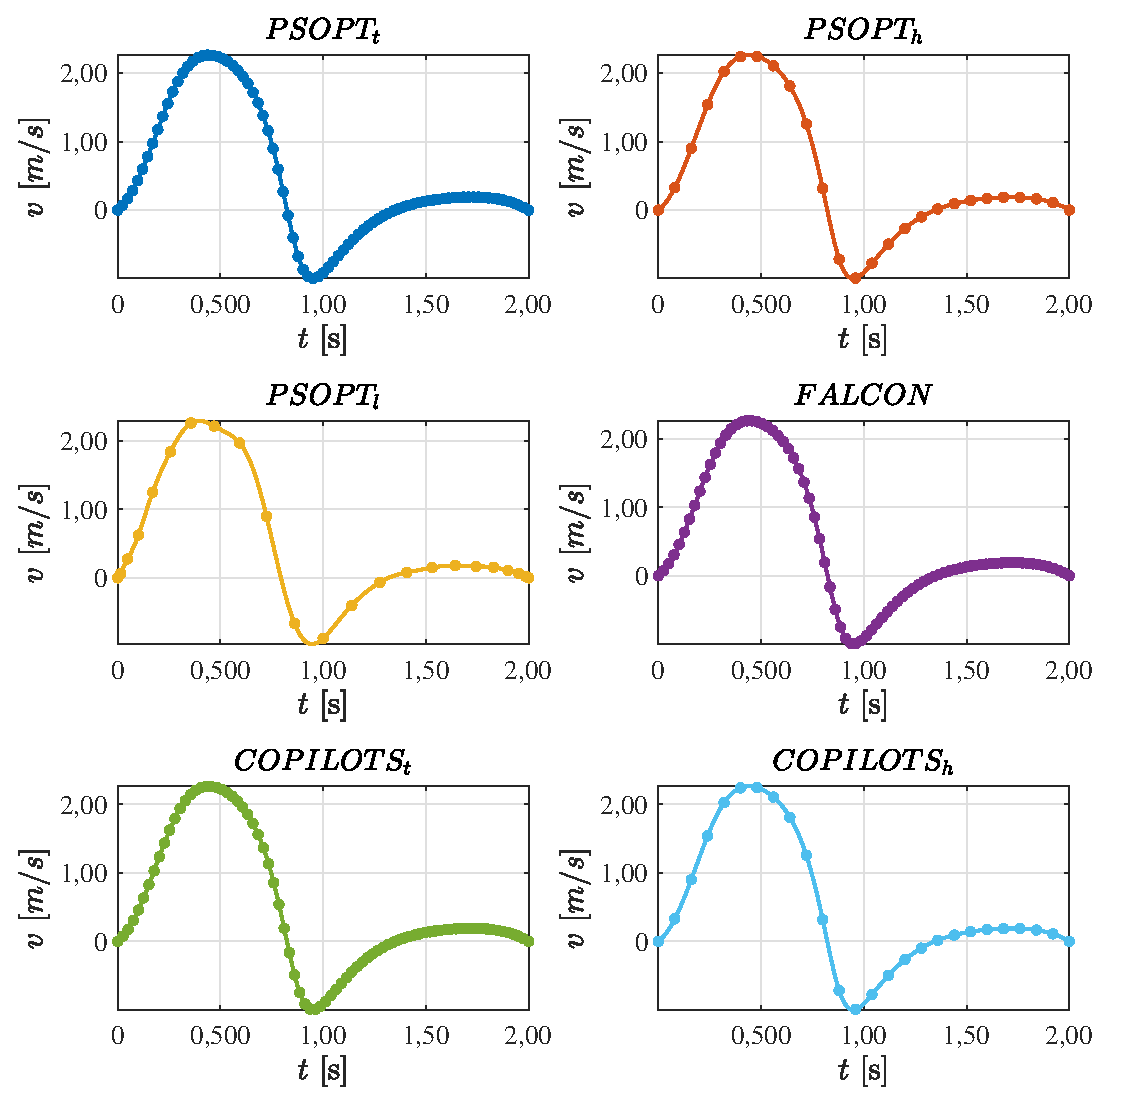
\includegraphics[scale=0.7]{fig/resultados/penduloInvertido/traj/x/v}
	\captionof{figure}[Variável de estado $v(t)$ para o problema do pêndulo]{Variável de estado $v(t)$ para o problema do pêndulo. Os pontos representam os valores discretizados e as linhas contínuas representam as trajetórias interpoladas.}
	\label{fig:penduloInvertido:x:v}
	\vspace{\onelineskip}
\end{minipage}

\noindent
\begin{minipage}{\textwidth}
	\vspace{\onelineskip}
	\centering
	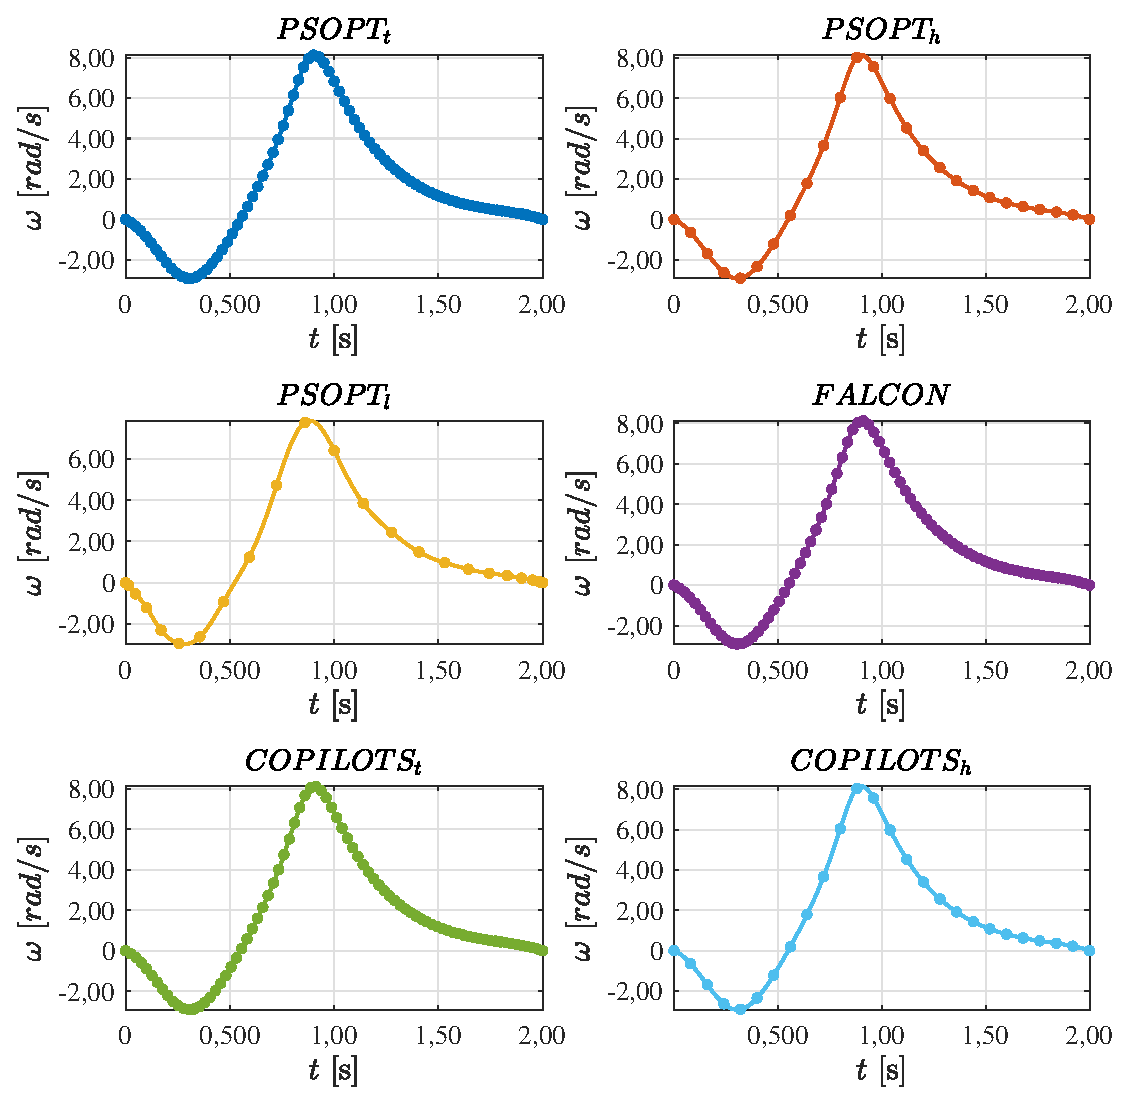
\includegraphics[scale=0.7]{fig/resultados/penduloInvertido/traj/x/omega}
	\captionof{figure}[Variável de estado $\omega(t)$ para o problema do pêndulo]{Variável de estado $\omega(t)$ para o problema do pêndulo. Os pontos representam os valores discretizados e as linhas contínuas representam as trajetórias interpoladas.}
	\label{fig:penduloInvertido:x:omega}
	\vspace{\onelineskip}
\end{minipage}

\noindent
\begin{minipage}{\textwidth}
	\vspace{\onelineskip}
	\centering
	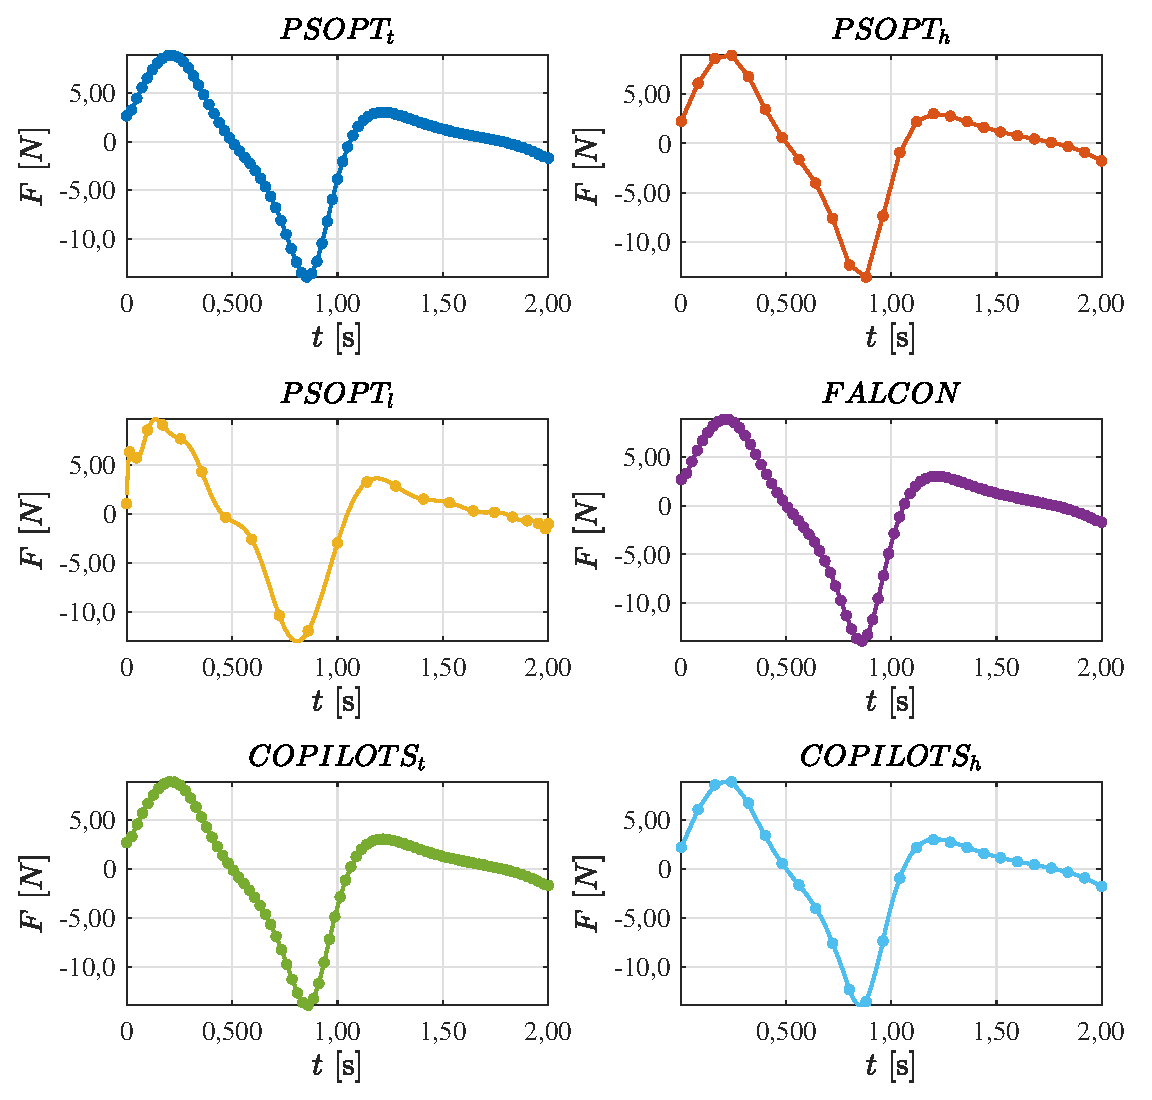
\includegraphics[scale=0.7]{fig/resultados/penduloInvertido/traj/u/F}
	\captionof{figure}[Variável de controle $F(t)$ para o problema do pêndulo]{Variável de controle $F(t)$ para o problema do pêndulo. Os pontos representam os valores discretizados e as linhas contínuas representam as trajetórias interpoladas.}
	\label{fig:penduloInvertido:u:F}
	\vspace{\onelineskip}
\end{minipage}

\todo[inline, color=pink, size=normalsize]{Análise das trajetórias}

\todo[inline, color=pink, size=normalsize]{Apresentação dos gráficos de trajetória complexos caso haja}

Já a Figura \ref{fig:penduloInvertido:avancado} apresenta a  vista lateral do pêndulo invertido, na qual são representadas algumas das posições durante a execução da manobra de \textit{swing-up}. A construção desse gráfico foi baseada nos resultados obtidos pelo $ COPILOTS_h $, o qual está associado ao menor valor de $ J^* $. Vale ressaltar que a posição da extremidade do pêndulo $ \big( x_e(t), y_e(t) \big) $ pode ser determinada com base nas relações $ x_e(t) = d(t) + l \, \sin\big( \theta(t) \big) $ e $ y_e(t) = l \, \cos \big( \theta(t) \big) $. Assim sendo, os pontos nesta figura representam os $ \big( x_e(t), y_e(t) \big) $ obtidos a partir dos valores calculados por $ d(t) $ e $ \theta(t) $ nos nós de colocação, enquanto a linha continua que conecta esses pontos representa a trajetória computada com base nas trajetórias apresentadas nas Figuras \ref{fig:penduloInvertido:x:d} e \ref{fig:penduloInvertido:x:theta}.

\noindent
\begin{minipage}{\textwidth}
	\vspace{\onelineskip}
	\centering
	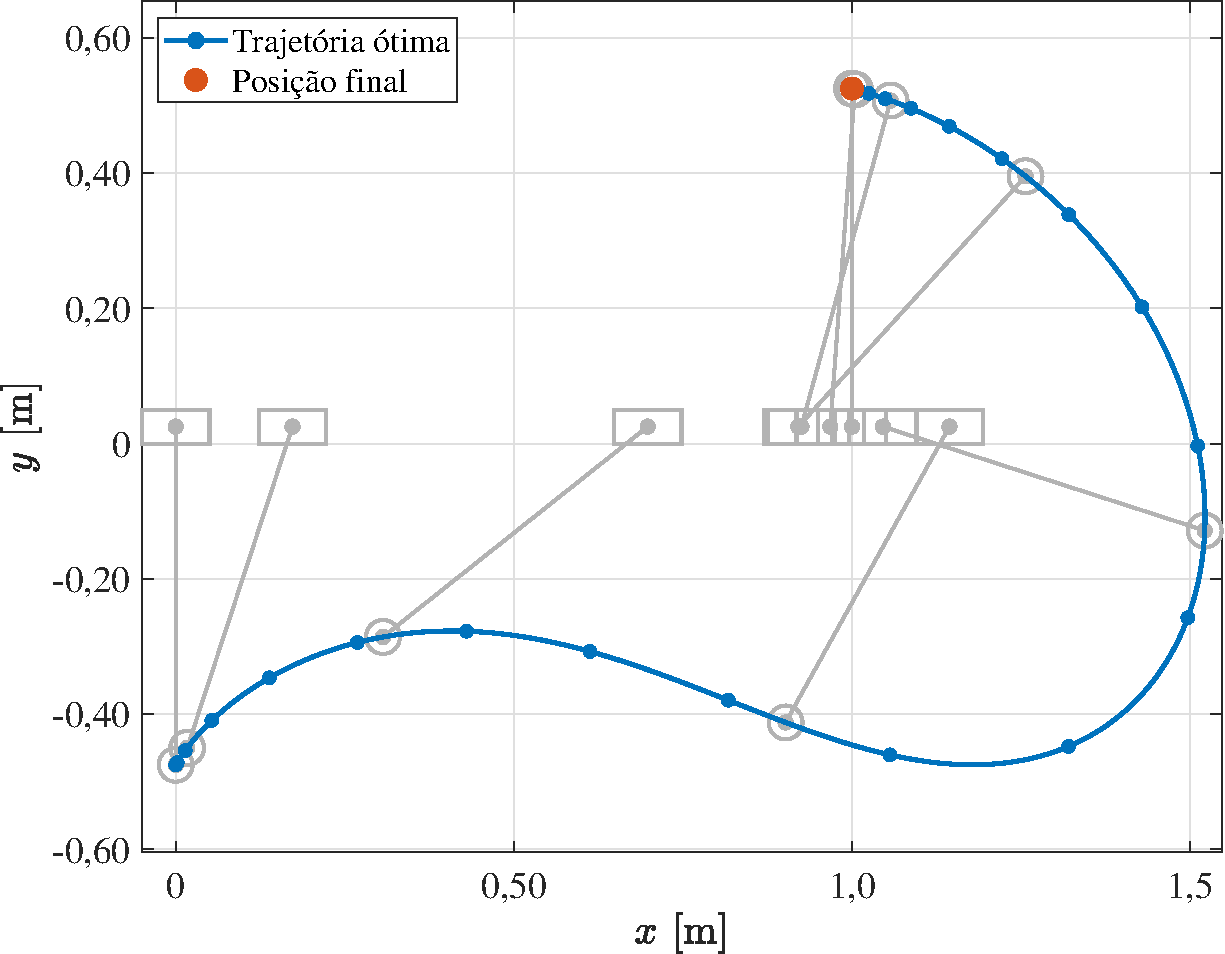
\includegraphics[scale=0.5]{fig/resultados/penduloInvertido/obs/adv}
	\captionof{figure}[Algumas posições do pêndulo invertido durante a execução da manobra de \textit{swing-up}]{Algumas posições do pêndulo invertido durante a execução da manobra de \textit{swing-up}.}
	\label{fig:penduloInvertido:avancado}
	\vspace{\onelineskip}
\end{minipage}

\todo[inline, color=pink, size=normalsize]{Introdução dos resultados $ t_p \times N $ e $ n_{aval} \times N $}

Para avalar a influência do número de nós de colocação no tempo de processamento e no número de avaliações da função objetivo são apresentadas nas Figuras \ref{fig:penduloInvertido:sensibilidade:t} e \ref{fig:penduloInvertido:sensibilidade:naval}. Nestes gráficos são apresentadas as variações: $ \Delta t_p = \max\{t_p\} - \min\{t_p\} $ e $ \Delta n_{aval} = \max\{n_{aval}\} - \min\{n_{aval}\} $. Os pontos nos gráficos representam os valores atribuídos a $ t_p $ (e a $ n_{aval} $) para cada um dos $ N $ considerados, enquanto as linhas contínuas representam curvas de tendência, obtidas por meio de regressões lineares, em que $R^2$ é o coeficiente de determinação. Os valores de $ N $ empregados na geração desses resultados são iguais àqueles considerados na computação da relação entre $ J^* $ e $ N $.

Nestas figuras é possível verificar que, de forma geral, ambos os valores de $ t_p $ e de $ n_{aval} $ aumentam com o incremento no valor do número de nós de colocação, conforme esperado. Além disso, em todas as configurações analisadas, os resultados obtidos pelo $ FALCON $ se mostram pouco sensíveis ao aumento de $ N $ em relação ao tempo e ao número de avaliações da função objetivo, conforme observado para $ \Delta t_p $ e $ \Delta n_{aval} $. Tal comportamento pode ser justificado pelo uso de informações simbólicas, o que na prática, facilita o cômputo de gradientes, necessários para a resolução do PPNL correspondente. Por outro lado, os valores de $ t_p $ e de $ n_{aval} $ associados ao $ COPILOTS $ se mostraram consideravelmente mais sensíveis ao aumento de $ N $ com relação as outras abordagens, conforme constatado avaliando-se $ \Delta t_p $ e $ \Delta n_{aval} $. Para este caso, imagina-se que estes valores elevados com relação à outras abordagens esteja relacionado a metodologia empregada para a resolução do PPNL associado. 

Já o tempo de processamento associado ao $ PSOPT_l $ se mostrou mais sensível ao aumento de $ N $ em relação ao $ PSOPT_t $ e ao $ PSOPT_h $. No entanto, os valores de $ n_{aval} $ associados ao $ PSOPT_t $, ao $ PSOPT_h $ e ao $ PSOPT_l $ se mostraram igualmente sensíveis ao aumento de $ N $, conforme pode ser observado ao se comparar os valores de $ \Delta n_{aval} $ para cada um. Para alguns dos $ N $ considerados, é possível verificar picos nos $ n_{aval} $ associados ao $ PSOPT_t $ e ao $ PSOPT_h $, o que justifica os baixos $ R^2 $ atribuídos a esses métodos. A presença desses picos pode ser justificada pela forma como cada pacote realiza a sua inicialização. Além disso, picos bastante similares podem ser observados nos valores de $ t_p $ e de $ n_{aval} $ associados ao $ COPILOTS_t $.

\noindent
\begin{minipage}{\textwidth}
	\vspace{\onelineskip}
	\centering
	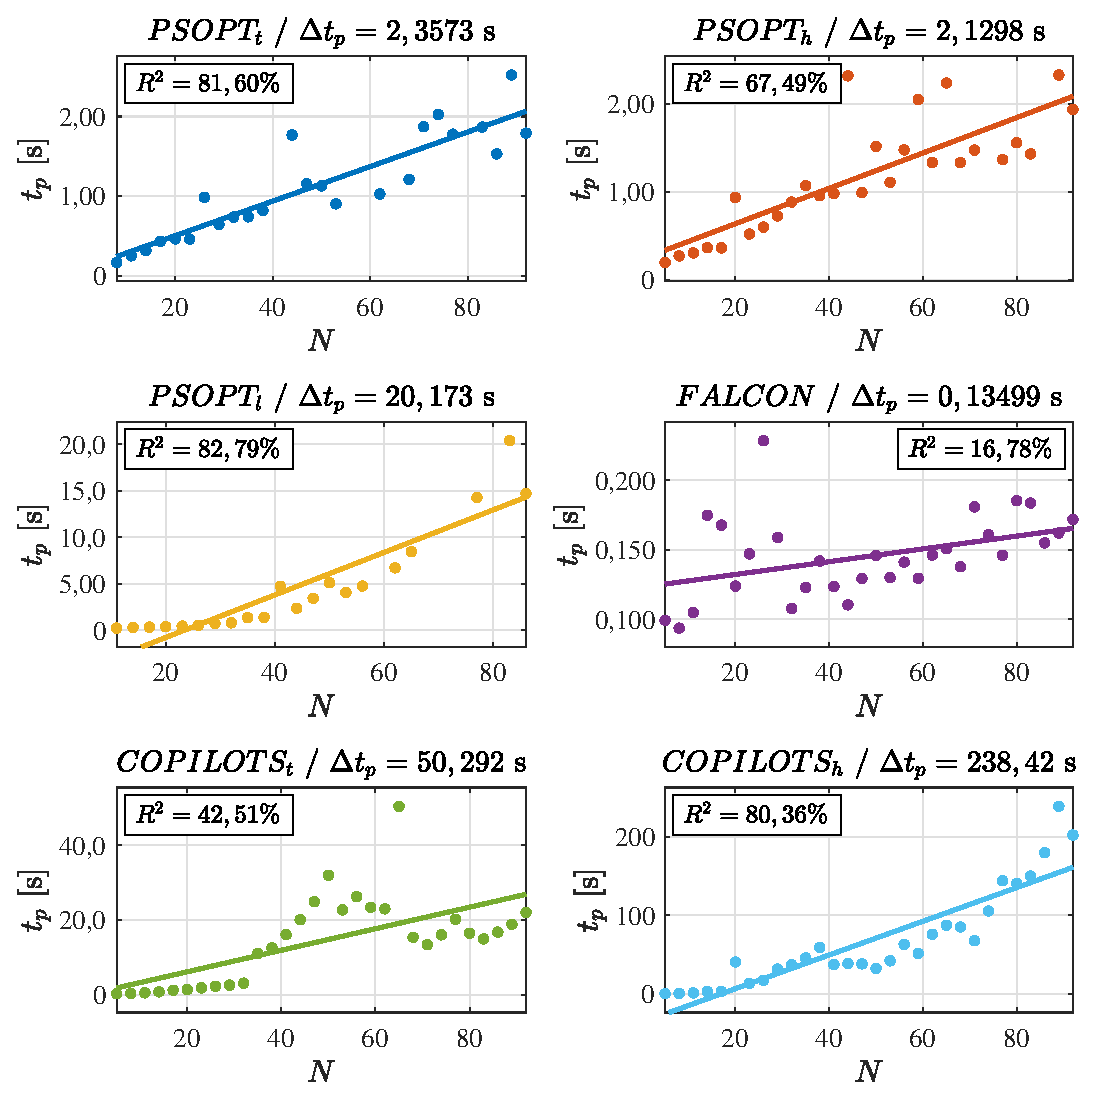
\includegraphics[scale=0.7]{fig/resultados/penduloInvertido/sens/t}
	\captionof{figure}[Relação entre o tempo de processamento e o número de nós de colocação para o problema do pêndulo invertido]{Relação entre o tempo de processamento $ t_p $ e o número de nós de colocação $ N $ para o problema do pêndulo invertido.}
	\label{fig:penduloInvertido:sensibilidade:t}
	\vspace{\onelineskip}
\end{minipage}

A Figura \ref{fig:penduloInvertido:sensibilidade:J} apresenta um comportamento diferente do esperado, isto é; espera-se que $ J^* $ diminua com o crescimento de $ N $, no entanto, para $ N < 14 $, verifica-se que ocorre o oposto. Anteriormente foi apresentada uma justificativa que leva em consideração o número de nós de colocação bem como o atendimento das restrições. Para explicar tal comportamento do ponto de vista matemático, serão avaliadas estratégias para a integração da função objetivo $ J $.   

Como a solução analítica do estudo de caso não é conhecida  \cite{kelly_introduction_2017}, será considerado como solução de referência aquela obtida usando o $ FALCON $ para $ N = 2000 $. Este foi escolhido por apresentar um comportamento suave para a variável de controle. De posse deste perfil, pode determinar o valor do referido objetivo.

\noindent
\begin{minipage}{\textwidth}
	\vspace{\onelineskip}
	\centering
	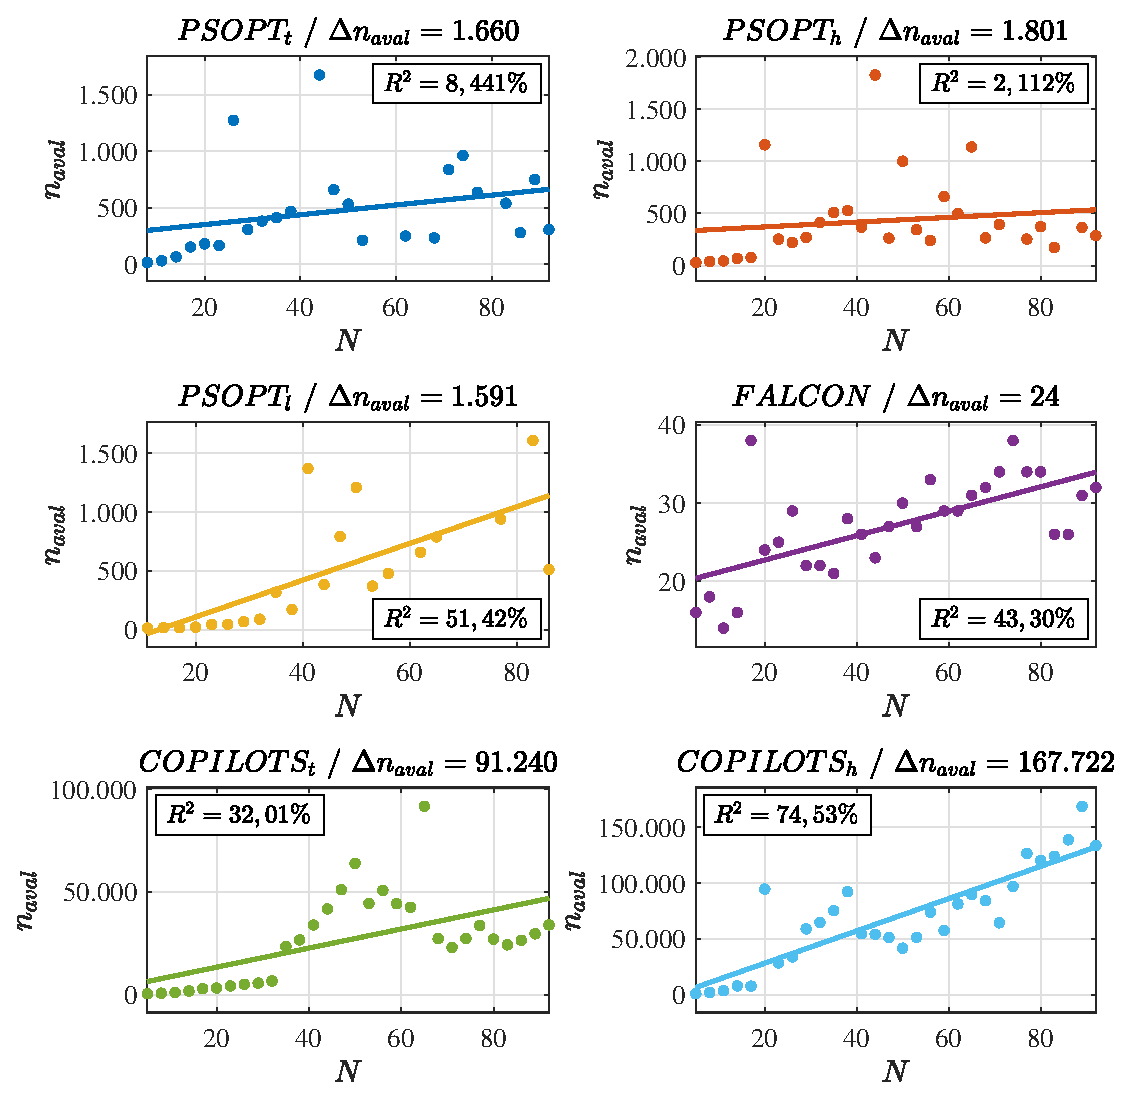
\includegraphics[scale=0.7]{fig/resultados/penduloInvertido/sens/eval}
	\captionof{figure}[Relação entre o número de avaliações da função objetivo e o número de nós de colocação para o problema do pêndulo invertido]{Relação entre o número de avaliações da função objetivo $ n_{aval} $ e o número de nós de colocação $ N $ para o problema do pêndulo invertido.}
	\label{fig:penduloInvertido:sensibilidade:naval}
	\vspace{\onelineskip}
\end{minipage}

\todo[inline, color=pink, size=normalsize]{Análise dos resultados $ t_p \times N $ e $ n_{aval} \times N $}

Ao se aplicar colocação trapezoidal, o cálculo da integral associada ao custo é realizada via uso de quadratura trapezoidal. As Figuras \ref{fig:penduloInvertido:trap:N=7}, \ref{fig:penduloInvertido:trap:N=9} e \ref{fig:penduloInvertido:trap:N=11} apresentam as aproximações lineares nas quais se baseia a computação de $ \int_{0}^{t_f} F^2(t) dt $ considerando $ N = 7 $, $ N = 9 $ e $ N = 11 $, respectivamente. Nota-se que o maior pico de $ F^2(t) $, que ocorre em $ t = 0,85 $ s, não é capturado para pequenos valores de $ N $. Desta forma, o valor atribuído a $ \int_{0}^{t_f} F^2(t) dt $ via quadratura trapezoidal acaba sendo bem menor que o valor verdadeiro, o que justifica os baixos $ J^* $ observados para $ N < 14 $, conforme ilustrado na Figura \ref{fig:penduloInvertido:sensibilidade:J}. 

Já na Figura \ref{fig:penduloInvertido:trap:NvsJ} é apresentada a relação entre o valor atribuído a $ \int_{0}^{t_f} F^2(t) dt $ via  quadratura trapezoidal e o número de nós de colocação $ N $. Como esperado, nota-se que o valor de $ J $ tende a estabilizar e convergir para a solução ótimo à medida que $ N $ cresce. Além disso, observa-se que tal convergência ocorre para $ N > 12 $, o que justifica os resultados obtidos conforme a Figura \ref{fig:penduloInvertido:sensibilidade:J}. 

\noindent	
\begin{minipage}{\textwidth}
	\vspace{\onelineskip}
	\centering
	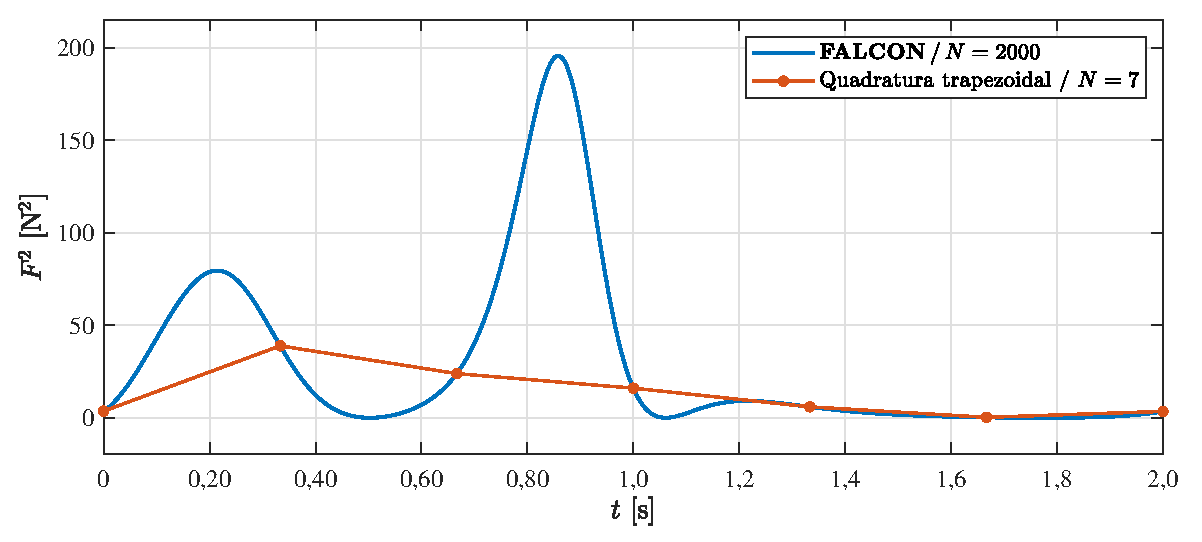
\includegraphics[scale=0.7]{fig/resultados/penduloInvertido/obs/trap/N=7}
	\captionof{figure}[Aproximações lineares para a avaliação de integrais usando quadratura trapezoidal ($ N = 7 $) no $ FALCON $]{Aproximações lineares para a avaliação de integrais usando quadratura trapezoidal ($ N = 7 $) no $ FALCON $.}
	\label{fig:penduloInvertido:trap:N=7}
	\vspace{\onelineskip}
\end{minipage}

\noindent	
\begin{minipage}{\textwidth}
	\vspace{\onelineskip}
	\centering
	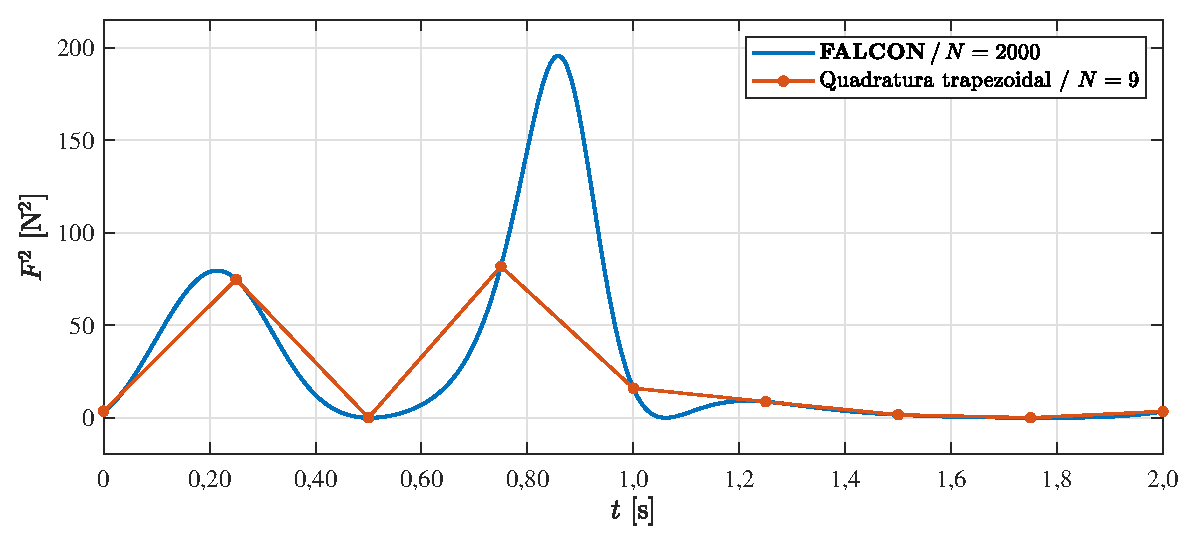
\includegraphics[scale=0.7]{fig/resultados/penduloInvertido/obs/trap/N=9}
	\captionof{figure}[Aproximações lineares para a avaliação de integrais usando quadratura trapezoidal ($ N = 9 $) no $ FALCON $]{Aproximações lineares para a avaliação de integrais usando quadratura trapezoidal ($ N = 9 $) no $ FALCON $.}
	\label{fig:penduloInvertido:trap:N=9}
	\vspace{\onelineskip}
\end{minipage}

Analogamente, é possível analisar os resultados obtidos considerando a colocação Hermite-Simpson. Para essa finalidade, nas Figuras \ref{fig:penduloInvertido:hersim:N=7}, \ref{fig:penduloInvertido:hersim:N=9} e \ref{fig:penduloInvertido:hersim:N=11} são representadas as aproximações quadráticas nas quais se baseia o cálculo de $ \int_{0}^{t_f} F^2(t) dt $ via quadratura de Simpson considerando $ N = 7 $, $ N = 9 $ e $ N = 11 $, respectivamente. Nesta figura, observa-se que o maior pico de $ F^2(t) $ não é satisfatoriamente representado na estimativa da integral em questão para $ N $ pequenos, o que pode justificar os menores valores de $J$ em relação à solução reportada na literatura. 

Na Figura \ref{fig:penduloInvertido:hersim:NvsJ} é apresentada a relação entre o valor da $ \int_{0}^{t_f} F^2(t) dt $ via quadratura de Simpson em função do parâmetro $ N $. Como esperado, o aumento no valor deste parâmetro implica na melhor aproximação da integral, o que na prática implica em uma melhor precisão. Neste caso, observa-se que tal convergência ocorre para $ N > 16 $, o que justifica os resultados verificados quando avalia-se a relação entre $ N $ e $ J^* $ apresentado na Figura \ref{fig:penduloInvertido:sensibilidade:J}.

Em resumo, a qualidade da solução encontrada em qualquer procedimento numérico sempre é função dos parâmetros que caracterizam a metodologia, bem como do nível de sofisticação da abordagem numérica empregada. No 
PCO isso não é diferente, isto é; a qualidade da solução também é função do nível de discretização informado pelo usuário (ou computado pela rotina considerada). Neste caso, sempre é importante realizar a análise de sensibilidade no que tange o efeito do número de nós ou pontos de colocação empregados.

\noindent	
\begin{minipage}{\textwidth}
	\vspace{\onelineskip}
	\centering
	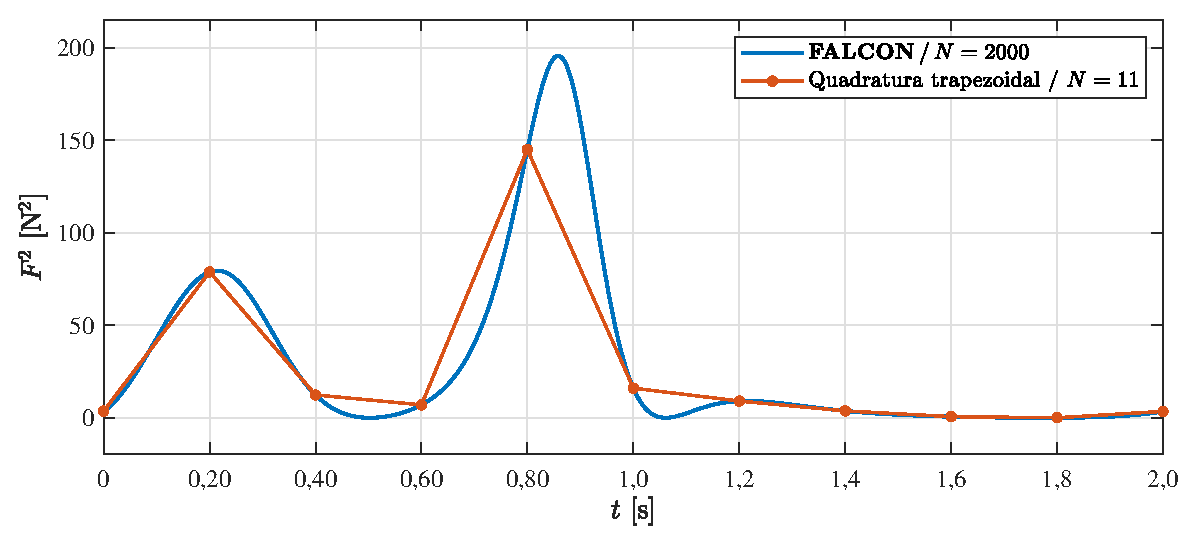
\includegraphics[scale=0.7]{fig/resultados/penduloInvertido/obs/trap/N=11}
	\captionof{figure}[Aproximações lineares para a avaliação de integrais usando quadratura trapezoidal ($ N = 11 $) no $ FALCON $]{Aproximações lineares para a avaliação de integrais usando quadratura trapezoidal ($ N = 11 $) no $ FALCON $.}
	\label{fig:penduloInvertido:trap:N=11}
	\vspace{\onelineskip}
\end{minipage}

\noindent	
\begin{minipage}{\textwidth}
	\vspace{\onelineskip}
	\centering
	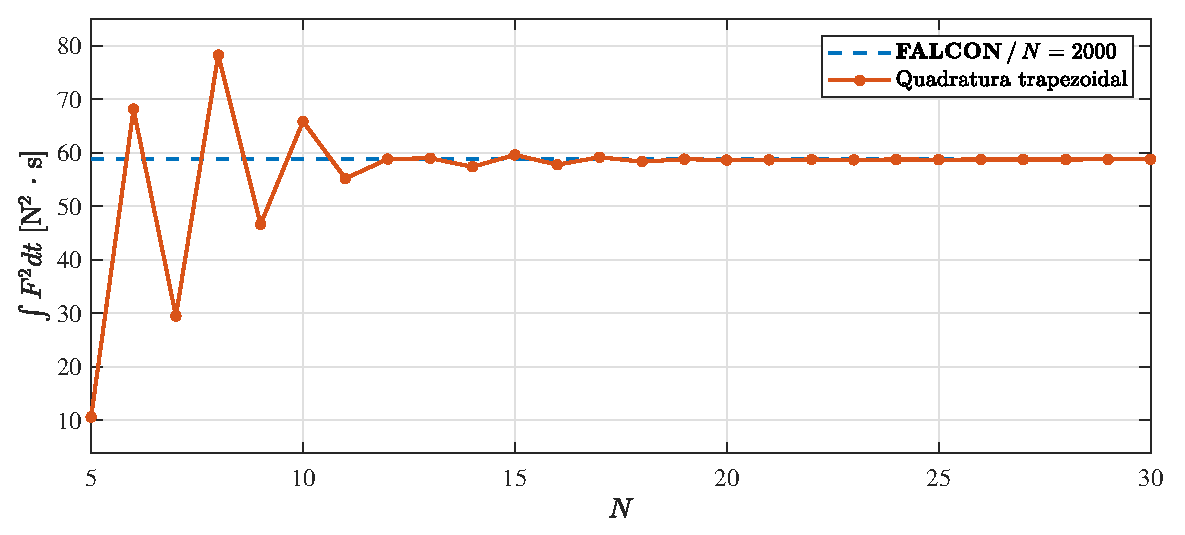
\includegraphics[scale=0.7]{fig/resultados/penduloInvertido/obs/trap/NvsJ}
	\captionof{figure}[Relação entre o valor atribuído a função objetivo via quadratura trapezoidal em função do número de nós de colocação]{Relação entre o valor atribuído a função objetivo via quadratura trapezoidal em função do número de nós de colocação.}
	\label{fig:penduloInvertido:trap:NvsJ}
	\vspace{\onelineskip}
\end{minipage}

\noindent	
\begin{minipage}{\textwidth}
	\vspace{\onelineskip}
	\centering
	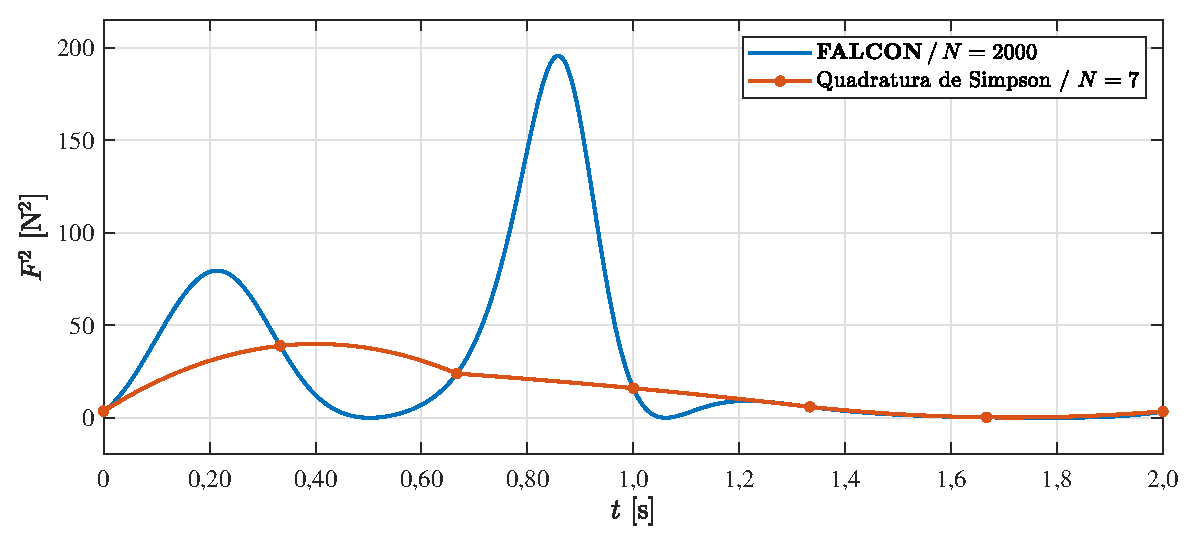
\includegraphics[scale=0.7]{fig/resultados/penduloInvertido/obs/hersim/N=7}
	\captionof{figure}[Função objetivo via quadratura de Simpson para o problema do pêndulo invertido ($N$=7)]{Função objetivo via quadratura de Simpson para o problema do pêndulo invertido ($N$=7).}
	\label{fig:penduloInvertido:hersim:N=7}
	\vspace{\onelineskip}
\end{minipage}

\noindent	
\begin{minipage}{\textwidth}
	\vspace{\onelineskip}
	\centering
	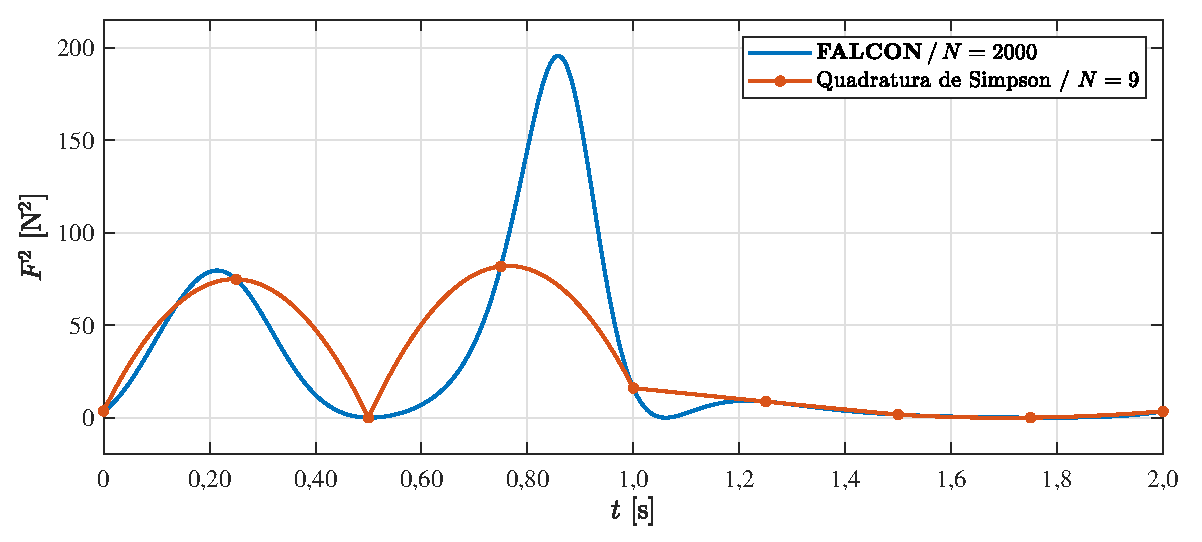
\includegraphics[scale=0.7]{fig/resultados/penduloInvertido/obs/hersim/N=9}
	\captionof{figure}[Função objetivo via quadratura de Simpson para o problema do pêndulo invertido ($N$=9)]{Função objetivo via quadratura de Simpson para o problema do pêndulo invertido ($N$=9).}
	\label{fig:penduloInvertido:hersim:N=9}
	\vspace{\onelineskip}
\end{minipage}

\noindent	
\begin{minipage}{\textwidth}
	\vspace{\onelineskip}
	\centering
	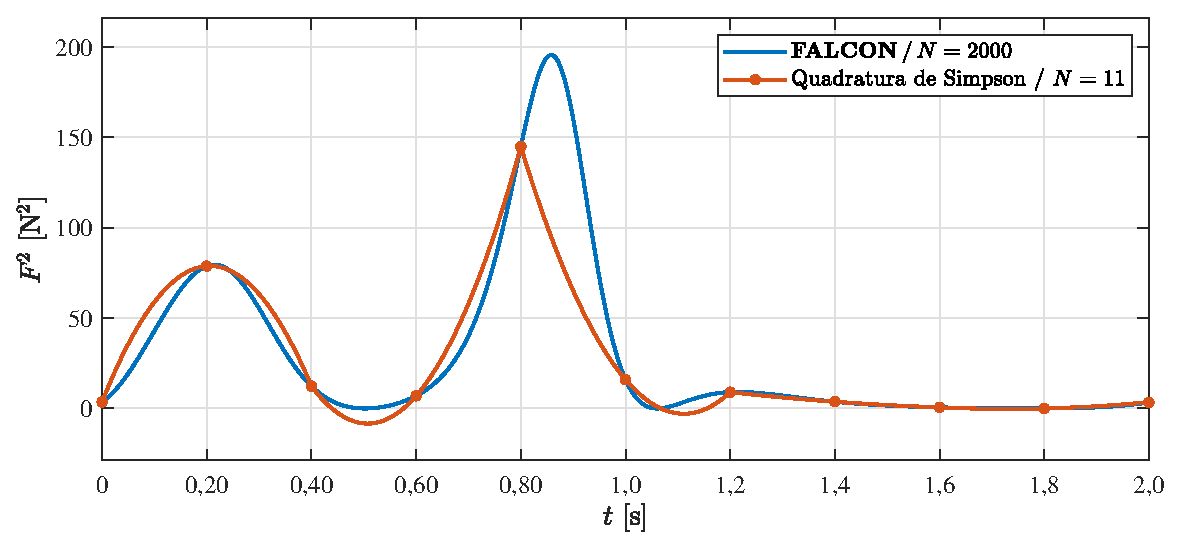
\includegraphics[scale=0.7]{fig/resultados/penduloInvertido/obs/hersim/N=11}
	\captionof{figure}[Função objetivo via quadratura de Simpson para o problema do pêndulo invertido ($N$=11)]{Função objetivo via quadratura de Simpson para o problema do pêndulo invertido ($N$=11).}
	\label{fig:penduloInvertido:hersim:N=11}
	\vspace{\onelineskip}
\end{minipage}

\noindent	
\begin{minipage}{\textwidth}
	\vspace{\onelineskip}
	\centering
	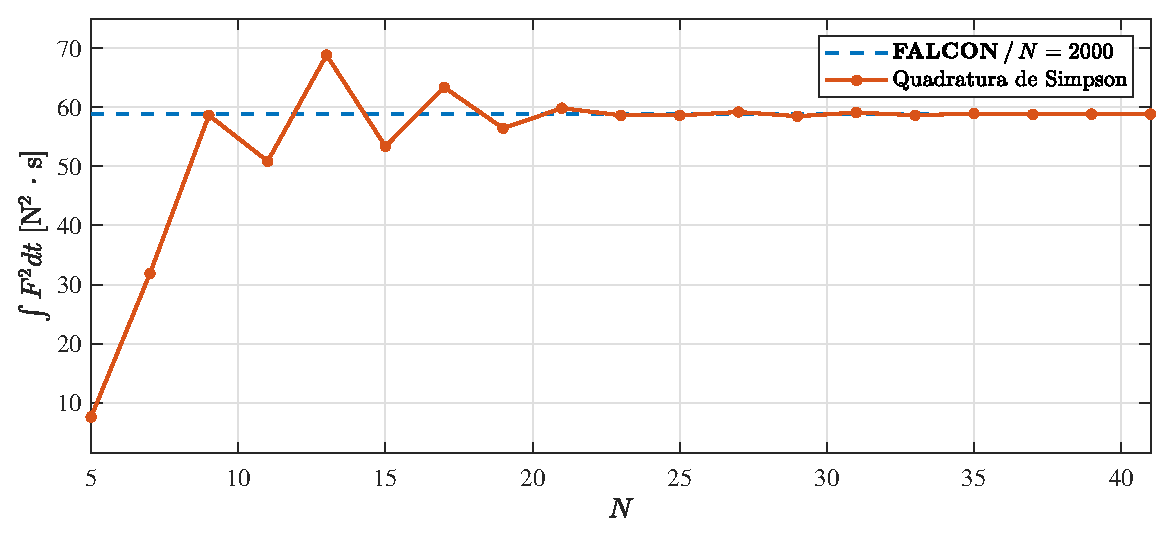
\includegraphics[scale=0.7]{fig/resultados/penduloInvertido/obs/hersim/NvsJ}
	\captionof{figure}[Relação entre o valor da função objetivo via quadratura de Simpson e o número de nós de colocação para o problema do pêndulo invertido]{Relação entre o valor da função objetivo via quadratura de Simpson e o número de nós de colocação para o problema do pêndulo invertido.}
	\label{fig:penduloInvertido:hersim:NvsJ}
	\vspace{\onelineskip}
\end{minipage}
